\documentclass[a4paper,12pt]{article}
\usepackage[chorded]{songs}
\usepackage{graphicx}
% \usepackage[
% % set width and height to a5 width and height + 6mm
% width=154truemm, height=216truemm,
% % use any combination of these options to add different cut markings
% cam, axes, frame, cross,
% % set the type of TeX renderer you use
% pdftex,
% % center the contents
% center
% ]{crop}


\songcolumns{2}
% \columnsep=0.4cm

\noversenumbers
\setlength{\songnumwidth}{0.5cm}
%\renewcommand{\lyricfont}{\sffamily\small}
\renewcommand{\chorusfont}{\it}
% \renewcommand{\snumbgcolor}{red}
\renewcommand{\printchord}[1]{\rmfamily\bf#1}
\versesep=12pt plus 2pt minus 2pt

\setlength{\cbarwidth}{0pt}
\setlength{\sbarheight}{0pt}

%\setlength{\versesep}{0pt}
%\setlength{\chordsep}{0pt}

\usepackage{geometry}
\geometry{
	a5paper,
	% total={170mm,257mm},
	left=5mm,
	top=10mm,
	right=5mm,
	bottom=3mm
}

\baselineadj=-10pt plus 1pt minus 0pt
%\renewcommand{\clineparams}{
%	\baselineskip=15pt
%	\lineskiplimit=5pt
%	\lineskip=1pt
%}

\newindex{mainindex}{idxfile}
\begin{document}
	\begin{figure}
		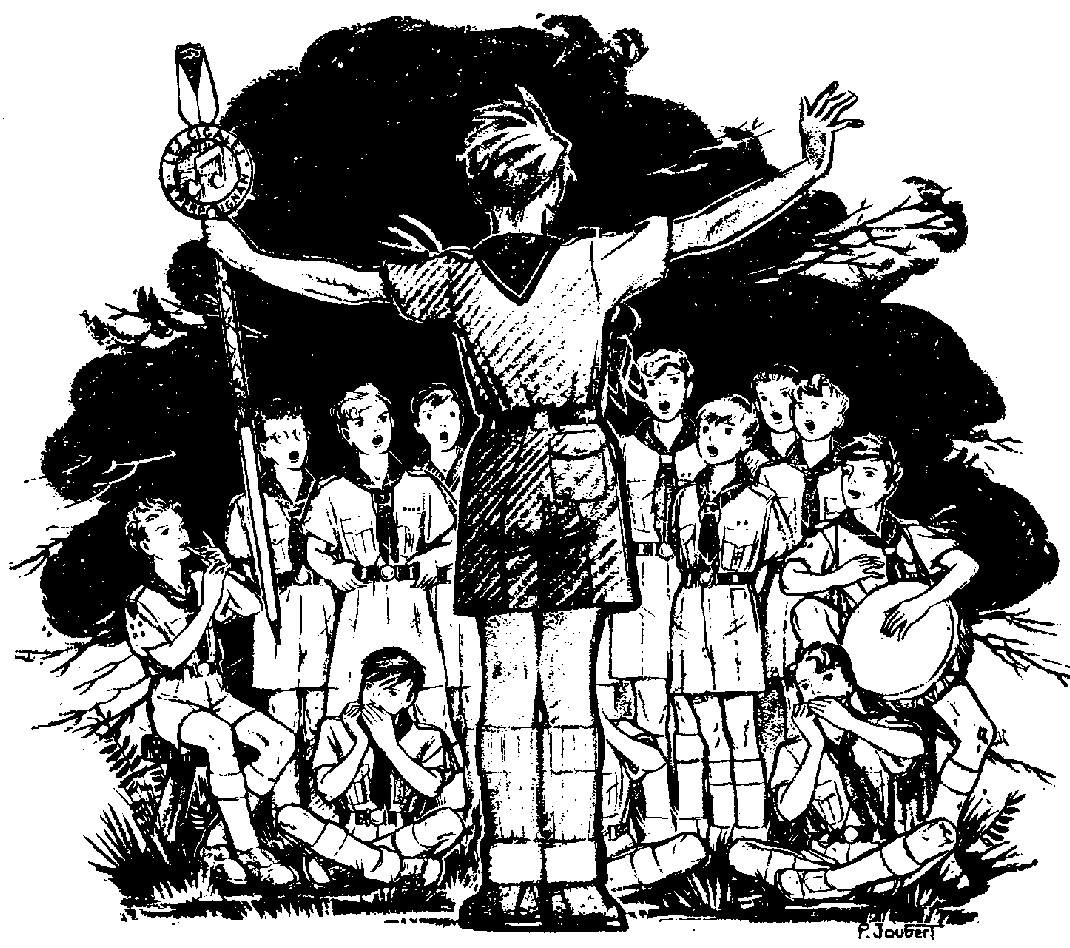
\includegraphics[width=\linewidth]{titre.jpg}
	\end{figure}
	\newpage

	\showindex[2]{Index alphabétique}{mainindex}
	
	\begin{songs}{}
		\beginsong{1987}[by={Calogero (2017)}]
		
		\beginverse
		\[D]Tu t'souviens  
		\[G]Les couleurs sur les baskets  
		\[Bm]Les crayons dans les cassettes  
		\[A]Je rembobine
		\endverse
		
		\beginverse
		Tu t'souviens  
		Tous ces rêves plein nos disquettes  
		À Paris c'était les States  
		1987
		\endverse
		
		\beginchorus
		Il \[D]y a certains jours où je reprends mon skate  
		\[A]Et je vais faire un tour en 1987  
		\[Bm]Il y a certains jours dans lesquels je me jette  
		\[F#m]Et je suis de retour en 1987  
		\[G]Tu sais de tous ces jours y'a rien que je regrette  
		\[F#m]Mais parfois je retourne en 1987, en 87
		\endchorus
		
		\beginverse
		Tu t'souviens  
		Les survêts et les houppettes  
		Sabrina et 7 sur 7  
		Dans la cuisine c'était rien  
		Que 12 mois sur la planète  
		L'URSS, INXS  
		On chantait I want your sex
		\endverse
		
		\beginchorus
		Refrain
		\endchorus
		
		\beginverse
		Tu verras bien qu'un jour une chanson dans la tête  
		Tu l'auras à ton tour ton 1987  
		Tu verras bien qu'un jour une chanson dans la tête  
		Tu l'auras à ton tour ton 1987  
		C'est tout ce que je te souhaite  
		Tu l'auras à ton tour ton 1987  
		C'est tout ce que je te souhaite  
		Tu l'auras à ton tour ton 1987  
		C'est tout ce que je te souhaite  
		Tu l'auras à ton tour ton 1987  
		Tu te souviens
		\endverse
		
		\endsong
		
		\beginsong{99 Luftballons}[by={Nena (1983)}]
		\beginverse
		Hast du etwas Zeit für mich?  
		Dann singe ich ein Lied für dich  
		Von 99 Luftballons  
		Auf ihrem Weg zum Horizont  
		Denkst du vielleicht gerade an mich  
		Dann singe ich ein Lied für dich  
		Von 99 Luftballons  
		Und dass sowas von sowas kommt
		\endverse
		\beginverse
		99 Luftballons  
		Auf ihrem Weg zum Horizont  
		Hielt man für UFOs aus dem All  
		Darum schickte ein General  
		Eine Fliegerstaffel hinterher  
		Alarm zu geben, wenn es so wäre  
		Dabei waren da am Horizont  
		Nur 99 Luftballons
		\endverse
		\beginverse
		99 Düsenflieger  
		Jeder war ein großer Krieger  
		Hielten sich für Captain Kirk  
		Das gab ein großes Feuerwerk  
		Die Nachbarn haben nichts gerafft  
		Und fühlten sich gleich angemacht  
		Dabei schoss man am Horizont  
		Auf 99 Luftballons
		\endverse
		\beginverse
		99 Kriegsminister  
		Streichholz und Benzinkanister  
		Hielten sich für schlaue Leute  
		Witterten schon fette Beute  
		Riefen Krieg und wollten Macht  
		Mann, wer hätte das gedacht  
		Dass es einmal soweit kommt  
		Wegen 99 Luftballons
		\endverse
		\beginverse
		99 Jahre Krieg  
		Ließen keinen Platz für Sieger  
		Kriegsminister gibt es nicht mehr  
		Und auch keine Düsenflieger  
		Heute ziehe ich meine Runden  
		Sehe die Welt in Trümmern liegen  
		Habe einen Luftballon gefunden  
		Denke an dich und lasse ihn fliegen
		\endverse
		\endsong
		
	\beginsong{Les Copains d’abord}[by={Georges Brassens}]
	\beginverse
		Non, ce n’était pas le radeau de la Méduse, ce bateau
		Qu’on se le dise au fond des ports, dise au fond des ports
		Il naviguait en pèr’peinard sur la grand-mare des canards
		Et s’app’lait les Copains d’abord, les Copains d’abord
		\endverse
		\beginverse
		Ses "fluctuat nec mergitur", c’était pas d’la littérature
		N’en déplaise aux jeteurs de sort, aux jeteurs de sort
		Son capitaine et ses mat’lots, n’étaient pas des enfants 
		d’salauds
		Mais des amis franco de port, des copains d’abord
			\endverse
		\beginverse
		C’étaient pas des amis de luxe, des petits Castor et Pollux
		Des gens de Sodome et Gomorrhe, Sodome et Gomorrhe
		C’étaient pas des amis choisis, par Montaigne et La Boétie
		Sur le ventre ils se tapaient fort, les copains d’abord
			\endverse
		\beginverse
		C’étaient pas des anges non plus, l’Évangile, ils l’avaient pas lu
		Mais ils s’aimaient toutes voiles dehors toutes voiles dehors
		Jean, Pierre, Paul et compagnie, c’était leur seule litanie
		Leur credo, leur confiteor, aux copains d’abord
			\endverse
		\beginverse
		Au moindre coup de Trafalgar, c’est l’amitié qui prenait l’quart
		C’est elle qui leur montrait le nord, leur montrait le nord
		Et quand ils étaient en détresse qu’leurs bras lançaient des 
		S.O.S.
		On aurait dit des sémaphores, les copains d’abord
			\endverse
		\beginverse
		Au rendez-vous des bons copains, y’avait pas souvent de lapins
		Quand l’un d’entre eux manquait à bord, c’est qu’il était mort
		Oui, mais jamais, au grand jamais, son trou dans l’eau n’se 
		refermait
		Cent ans après, coquin de sort, il manquait encore
			\endverse
		\beginverse
		Des bateaux j’en ai pris beaucoup mais le seul qui ait tenu le 
		coup
		Qui n’ai jamais viré de bord, mais viré de bord
		Naviguait en père peinard sur la grand-mare des canards
		Et s’app’lait les Copains d’abord, les Copains d’abord
		\endverse
	\endsong
	\beginsong{À nos souvenirs}[by={Trois Cafés Gourmands}]
	\beginverse
	Regardez-\[Sol]nous, à \[Do]quinze ans sur cette \[Ré]photo\\
	On fait les \[Sol]fous, tous les \[Do]deux sur le même vé\[Ré]lo\\
	On s'est connus, \[Sol]toi et \[Do]moi bien avant nos \[Ré]mots\\
	On s'est per\[Sol]dus de \[Do]vue, trop \[Ré]tôt
	\endverse
	
	\beginchorus
	À nos souve\[Ré]nirs, à nos es\[Sol]poirs, à la \[Do]vie\\
	À nos souve\[Ré]nirs, à ces fous \[Sol]rires, à l'in\[Do]fini\\
	À l'amour, à \[Ré]nos nuits blanches, à nos dé\[Do]lires\\
	À nos souve\[Sol]nirs
	\endchorus
	\endsong
	\end{songs}
\end{document}

